%%TODO: IF THIS GETS IN, CITE MY THESIS (since I present an early version
%of this idea in my background and copied some text from there)

% Template for ICIP-2018 paper; to be used with:
%          spconf.sty  - ICASSP/ICIP LaTeX style file, and
%          IEEEbib.bst - IEEE bibliography style file.
% --------------------------------------------------------------------------
\documentclass{article}
\usepackage{spconf,amsmath,amssymb,amsfonts,amsthm,graphicx}


\graphicspath{{Figures/}}
\newcommand{\argmin}{\operatornamewithlimits{argmin}}
\newcommand{\argmax}{\operatornamewithlimits{argmax}}


\title{Topological Eulerian Synthesis of Slow Motion Periodic Videos}

%
% Single address.
% ---------------
\name{Author(s) Name(s)\thanks{Thanks to XYZ agency for funding.}}
\address{Author Affiliation(s)}
%
% For example:
% ------------
%\address{School\\
%	Department\\
%	Address}
%
% Two addresses (uncomment and modify for two-address case).
% ----------------------------------------------------------
%\twoauthors
%  {A. Author-one, B. Author-two\sthanks{Thanks to XYZ agency for funding.}}
%	{School A-B\\
%	Department A-B\\
%	Address A-B}
%  {C. Author-three, D. Author-four\sthanks{The fourth author performed the work
%	while at ...}}
%	{School C-D\\
%	Department C-D\\
%	Address C-D}
%
\begin{document}
%\ninept
%
\maketitle
%


\begin{abstract}

The majority of our pipeline is fully automated, using tools from topological data analysis in concert with nonlinear dimenison reduction to autotune the spatial and temporal scales of the period.

\end{abstract}
%
\begin{keywords}
One, two, three, four, five
\end{keywords}
%


\section{Introduction}
%Background, drift, noise, large motion, static pixels, scale finding, overall automation [fundamental frequency, etc].  Sliding window "time regularization"

Repetitive, periodic motions are ubiquitous in our world, such as animal locomotion (walking/flapping/slithering/swimming), mechanical motions (wheels spinning, pistons oscillating), biological rhythms (heartbeat, breathing), musical rhythms (drumming, feet tapping), etc.  In this work, we consider the problem of synthesizing a fine detail, ``slow motion'' template cycle of motion from a video of such a motion with many periods.  This fine detailed analysis can be applied, for example, to characterize subtle progressions of blood flow in the face during a heartbeat \cite{kumar2015distanceppg}.  Having access to a consensus template can also be used to visualize variations from cycle to cycle, such as in a repetitive automated action on an assembly line, where too much variation could indicate the onset of failure (TODO: citation), or in athletic activities for optimizing performance.

Our approach to slow motion templates is {\em Eulerian}; that is, we process the video pixel by pixel with no tracking.  Eulerian approaches for video synthesis are attractive due to their simplicity and ease of implementation.  For instance, a simple Fourier bandpass filtering and amplifying pixels can successfully elucidate subtle periodic motions in videos \cite{wu2012eulerian, wadhwa2013phase}.  Additionally, time domain Eulerian approaches have been used to synthesize infinitely playing ``video textures'' using random walks \cite{schodl2000video}, or to synthesize perfectly looping video templates after grouping pixels with similar periods together and devising a common period for all groups \cite{Liao2013VideoLoops,Liao2015VideoLoops}.  There are some pitfalls with Eulerian techniques, however.  Purely Eulerian amplification techniques are known to fail for large motions, and they also require the user to manually specify frequencies of interest \cite{wu2012eulerian, wadhwa2013phase}.  Furthermore, drift from period to period due to shaking and varying motions from cycle to cycle can present a problem, as can unrelated motion in the background \cite{stauffer1999adaptive}.

To address the problems with an Eulerian representation, we devise a geometric/topological Eulerian framework byconstructing {\em sliding window embeddings} of our videos (Section~\ref{sec:slidingwindow}).  Sliding window embeddings, or ``delay reconstructions,'' have found a diverse array of applications in activity recognition \cite{frank2010activity,venkataraman2016shape}, gene expression data \cite{perea2015sw1pers}, EEG analysis \cite{stam2005nonlinear, plesnik2014detection}, audio and music analysis \cite{herzel1994analysis,serra2009cross,bello2011measuring,traliemoebius}, video analysis \cite{tralie2017quasi}, and motion capture analysis \cite{venkataraman2016shape}.  Sliding window embeddings of periodic time series, in particular, form samples of a topological loop \cite{perea2015sliding}, as do generalized multivariate sliding windows on periodic video data, regardless of the type of motion present \cite{traliehigh, tralie2017quasi}.  Furthermore, as shown by the authors of \cite{tralie2017quasi}, sliding window embeddings on Eulerian videos provide a sort of ``time regularization,'' which can mitigate the effects of drift, leading to a cleaner loop.  Our geometric framework also allows us to use topological data analysis \cite{edelsbrunner2000topological,edelsbrunner2008persistent,edelsbrunner2010computational,carlsson2009topology,ghrist2014elementary} and fundamental frequency estimation \cite{Mcleod05asmarter} to autotune the temporal and spatial scales of the periodic motion, respectively, so that no user intervention is required.  Our embedding also makes it easy to assign each window a circular phase $\phi \in [0, 2\pi]$ using Laplacian Eigenmaps \cite{belkin2003laplacian}.  We then re-order the sliding windows by $\phi$ and exploit the sliding window structure to have different windows vote on the final pixels in each frame of the template, which further mitigates drift (Section~\ref{sec:cyclereordering}).  As an illustration, Figure~\ref{fig:ConceptFigure} shows an example of our technique on a sampled periodic time series (i.e. single pixel grayscale video).  There are only 12 samples per period in the original signal, so the details of each period coarse and noisy.  However, once they are re-sorted, we get a nice, fine-detailed representation of one period.  The extension of this technique to videos will be described in detail in Section~\ref{sec:methods}.


Many prior works use a combination of sliding window embeddings and topological data analysis, such as detecting the Lorenz attractor \cite{de2012topological}, quantifying circadian rhythms in gene expression data \cite{perea2015sliding}, detecting chatter in mechanical systems \cite{khasawneh2016chatter}, detecting wheezing in audio \cite{emrani2014real}, quantifying periodic activites in motion capture data \cite{vejdemo2015cohomological, venkataraman2016persistent}, and quantifying vocal fold anomalies in video \cite{tralie2017quasi}, though we believe we are the first to use a sliding window + TDA framework to {\em synthesize} a new result.  Our use of the graph Laplcian to parameterize time series is also unique, though we are inspired by works that have used it to re-arrange images around a loop as a pre-processing step for structure from motion \cite{averbuch2015ringit}, and works which use vector diffusion maps to re-order the frames of microscope images a developing embryo around a loop \cite{dsilva2015diffusionvecordering}.  We use the combination of TDA + Laplacian eigenmaps as a simple alternative to the more complicated cohomology circular coordinates proposed by the authors of \cite{de2011persistent} and used on motion capture data \cite{vejdemo2015cohomological}.


\section{Slow Motion Templates}
\label{sec:methods}

\begin{figure*}
\centering
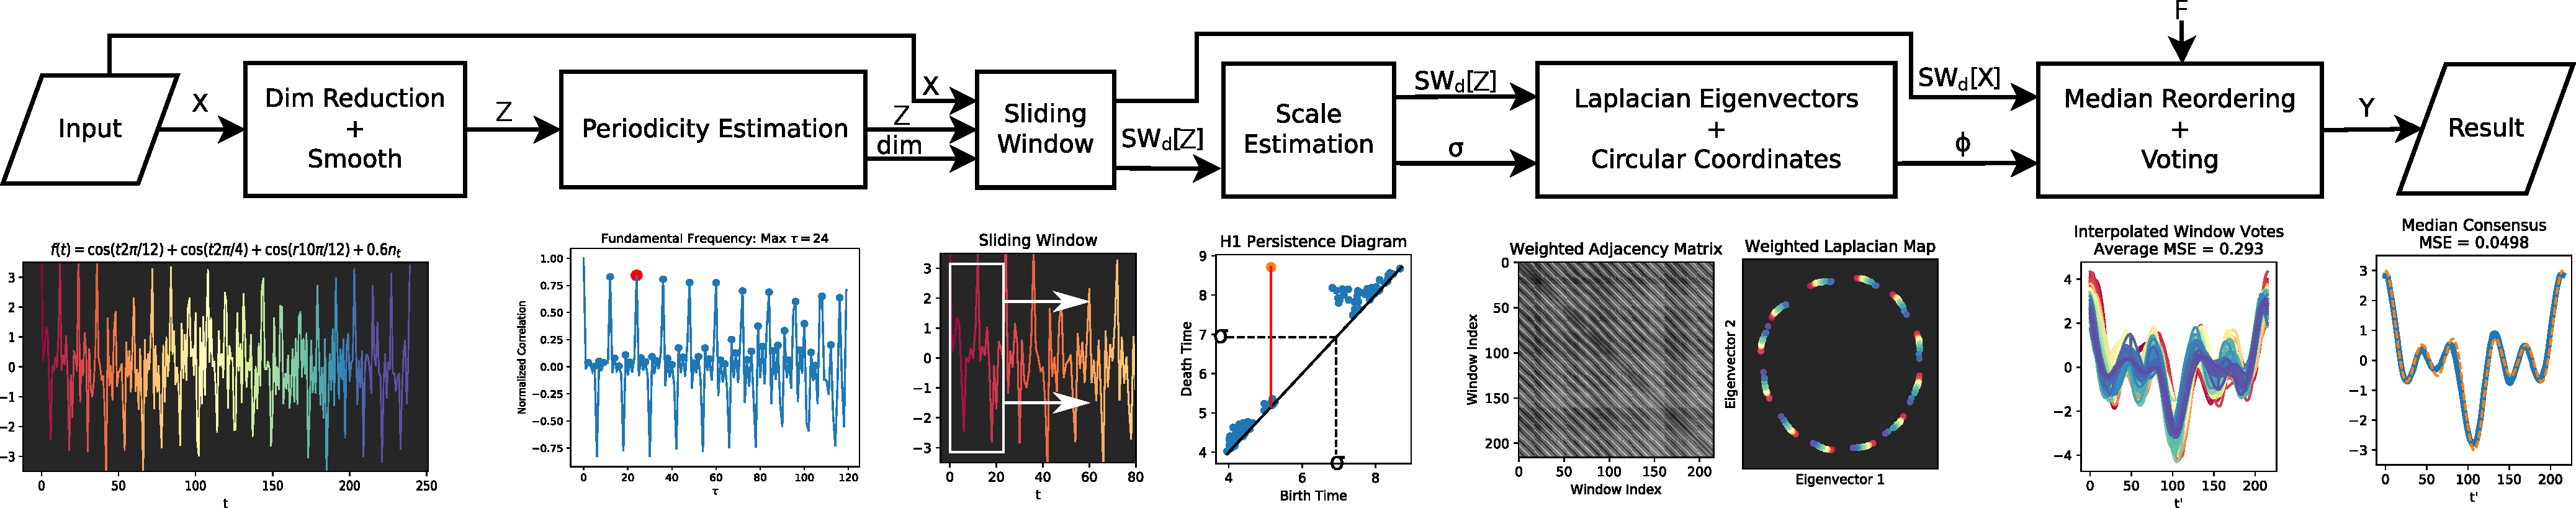
\includegraphics[width=\textwidth]{BlockDiagram.pdf}
\caption{An block diagram of our technique, illustrated by a 1D periodic time series with additive Gaussian noise ($n_t \in \mathcal{N}(0, 1)$).  We estimate the period to be 24 (a multiple of the fundamental frequency), and perform a 24-length sliding window embedding.  From this, we use the mean of the birth and death time of the largest persistence dot to autotune the scale $\sigma$ for the graph Laplacian, from which we derive circular coordinates $\phi$, which can be used to reorder the sliding windows and use them to vote on a final slow motion template.  The result is shown in the bottom rightmost plot, superimposed with a ground truth period shows as an orange dotted line.}
\label{fig:ConceptFigure}
\end{figure*}



We now describe our algorithm in several stages.  Throughout our discussion, we assume we are given 3 channel color videos with $W \times H$ resolution frames, so that each frame is a Euclidean vector in $\mathbb{R}^{W \times H \times 3}$.  For a video with $N$ frames, we flatten each frame to a 1D vector and stack them row wise along an $N \times 3WH$ matrix $X$.  Whenever we perform a linear operation on all of the pixels at once, we can use the SVD $X = USV^T$ to reduce memory and computational costs by working with $US$ in place of $X$, which is in $N$ dimensions instead of $3WH \gg N$ (similar processing was done in \cite{turk1991eigenfaces} and \cite{tralie2017quasi}).  The only nonlinear operation is the median operation (Section~\ref{sec:cyclereordering}), and we project back into pixel space using $V^T$ before taking the median.

\subsection{Sliding Window Embeddings}
\label{sec:slidingwindow}

Given a $W \times H$ video $X(t) \in \mathbb{R}^{3WH}$ indexed by time, the sliding window video embedding \cite{cao1998dynamics,traliehigh,tralie2017quasi} is defined as

\begin{equation}
SW_{d, \tau}[X(t)] = \left[ \begin{array}{c} X(t) \\ X(t + \tau) \\ \vdots \\ X(t + (d-1)\tau)  \end{array} \right] \in \mathbb{R}^{3WHd}
\end{equation}

where $\tau$ is a step size and $d$ is the dimension of the embedding.  In this work, we fix $\tau = 1$ for simplicity and drop $\tau$ in the subscript, and we also sample times $t$ only at integer frame indices.  As shown by Takens \cite{takens1981detecting}, a sliding window of dimension $d = 2m+1$ of even a single generic observation function (time series) of a dynamical system of intrinsic dimension $m$ is sufficient to reconstruct a topological embedding of the underlying trajectory in the original state space.  For periodic signals, this state space is a torus, and $d$ should be twice the number of harmonics present to injectively reconstruct loops on that torus \cite{perea2015sliding}.  The same is true of videos in general \cite{tralie2017quasi}.  Furthermore, the sliding window length $(d-1) \tau$, or simply $d-1$ in our case, maximizes the roundness of the embeddings when $d-1 = k T$ for some integer $k$, where $T$ is the fundamental period.  Since we will use topological data analysis (TDA) to find the scale of the loop, and since TDA measures roundness, it is important that we tune our window size to be an integer multiple of the period.  To do this, we perform 1D ISOMAP \cite{tenenbaum2000global} on the original frames of the video to generate a 1D ``surrogate signal,'' and we perform an autocorrelation-based fundamental frequency estimation \cite{Mcleod05asmarter} on this signal to estimate the period and, hence, the appropriate $d$.  This is quite similar to the diffusion maps + autocorrelation approach in \cite{tralie2017quasi} for analyzing periodic videos.  This estimation often returns integer multiples of the fundamental period, which is fine for our purposes.

\subsection{Laplacian Eigenmaps And Persistent Homology}
\label{sec:laplacian}

Since sliding window embeddings of periodic videos lie on a topological loop (a manifold which is an ``intrinsic circle''), this means that, at an appropriate scale, a nearest neighbors graph built on the sliding window point cloud will approximately be a circle graph.  To parameterize this graph, we turn to the graph Laplacian \cite{chung1997spectral}.  For a graph $G$ with $N$ vertices and an $N \times N$ symmetric adjacency matrix $A$, the graph Laplacian is defined as
\begin{equation}
L = D-A
\end{equation}
where $D_{ii} = \sum_{j = 1}^N A_{ij}, D_{i \neq j} = 0$ is the diagonal matrix.  Now let $d_{ij}: V \rightarrow \mathbb{R}^+$ be a nonnegative scalar function on the vertices of $G$.  Then the adjacency matrix correponding to the {\em unweighted} graph Laplacain, $A_{\epsilon}^u(d)$, is

\begin{equation}
A_{\epsilon}^u(d)_{ij} = \left\{ \begin{array}{cc} 1 & i \neq j, d_{ij} \leq \epsilon \\ 0 & \text{otherwise} \end{array} \right\}
\end{equation}

For a circle graph, where the $A_{ij} = 1$ if $|i-j| = 1$, $i=1, j=N$, and $j=1, i=N$, or zero otherwise, the eigenvectors spanning the image of the graph laplacian are 

\begin{equation}
v_{2k}[n] = \cos(2 \pi k n / N), v_{2k-1}[n] = \sin(2 \pi k n / N), k \geq 1
\end{equation}

%In other words, the graph Laplacian of an $N$-point circle graph recovers the $N$-dimensional discrete Fourier transform.

with corresponding eigenvalues $\lambda_k = 2 - 2 \cos(2 \pi k / N)$ (and $\lambda_0 = 0$ with corresponding eigenvector $v_0[n] = 1$).  When computing the eigenvectors of a circle graph numerically, therefore, $v_1$ and $v_2$ should be a sine and cosine, or orthogonal linear combinations therein.

TODO: Talk about circulant graphs instead



which means the first two nonzero eigenvectors should be a sine and cosine, or orthogonal linear combinations therein.  When plotted against each other, they make an approximate circle, and the arctangent of the two eigenvector coordinates at every window can be used to determine the {\em phase} of the corresponding window in the periodic signal.  The first sample of each window can then be re-sorted by phase.

Talk about autotuning with peristent homology, mention that it's the opposite of the approach in \cite{bendich2011improving}

Talk about how it can pick up on harmonics (e.g. jumping jacks), which is why this is important (talk about using prime 49)

\subsection{Cycle Reordering And Median Voting}
\label{sec:cyclereordering}



Advantage of Eulerian is that everything is linear (can use SVD to compress)

Interpolated windows can be projected back to pixel space one by one to save memory

\subsection{Sharpening Postprocessing}

The results of the median reordering can be blurry


\section{Experiments}

\subsection{Robustness Tests}
Robustness experiments

\subsection{Qualitative Results}
\begin{figure}[h!]
\centering
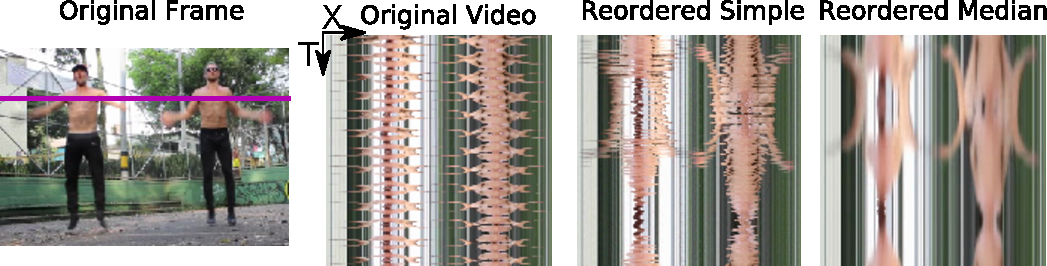
\includegraphics[width=\columnwidth]{XTSliceJumpingJacks.pdf}
\caption{An XT slice of a line of pixels (magenta line, upper left) over time for an input video of two men doing jumping jacks and for reordered videos with and without median consensus.}
\label{fig:XTSliceJumpingJacks}
\end{figure}

\begin{figure}[h!]
\centering
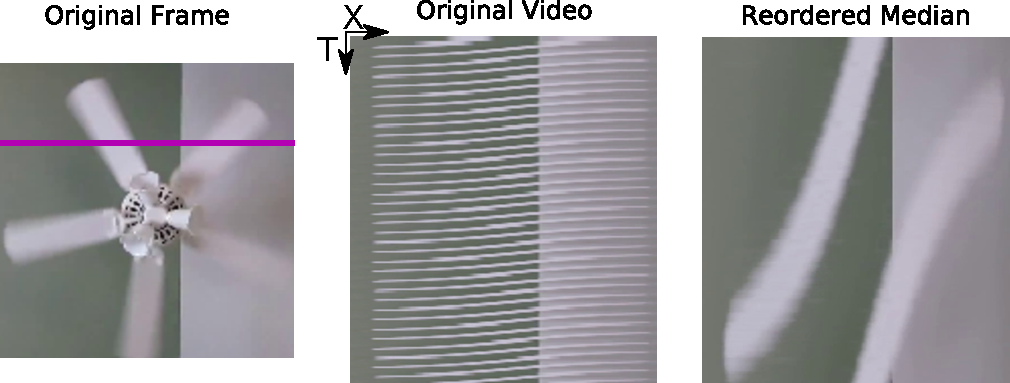
\includegraphics[width=\columnwidth]{XTSliceFan.pdf}
\caption{An XT slice of a line of pixels (magenta line, upper left) over time for an input video of a fan with only 6 frames per period and the corresponding median consensus reordered video.}
\label{fig:XTSliceFan}
\end{figure}

Figure~\ref{fig:XTSliceJumpingJacks} shows the difference between a simple reordering and a median consensus reordering.  Due to natural variation from cycle to cycle, the simple reordering has many temporal discontinuities when interleaving these cycles.  By contrast, the median voting is clean, and it has the added benefit of removing nonperiodic background components.

umping jacks 2 men, two exercise videos from \cite{levy2015live}, beating heart videos from \cite{traliehigh}, \cite{wu2012eulerian}, and \cite{wadhwa2013phase}.

\section{Discussion}

Since we rely on the theory and constructions in \cite{tralie2017quasi}, we are subject to similar constraints in the allowable motion and drift for our method to work well.  We note that Eulerian video magnification also degrades in the presence of too much drift \cite{wu2012eulerian, wadhwa2013phase}.


% References should be produced using the bibtex program from suitable
% BiBTeX files (here: strings, refs, manuals). The IEEEbib.bst bibliography
% style file from IEEE produces unsorted bibliography list.
% -------------------------------------------------------------------------
\bibliographystyle{IEEEbib}
\bibliography{refs}

\end{document}
